\documentclass{article}
\usepackage{graphicx}
\usepackage{hyperref}
%\usepackage{fancyhdr}
%\usepackage{lipsum} % For placeholder text
%\usepackage{cite}  % Optional: for citation styles
%\usepackage[backend=biber,style=numeric,sorting=none]{biblatex} % Use biblatex and sorting=none for continuous numbering
\usepackage[backend=biber,style=numeric,sorting=none]{biblatex} % Use biblatex and sorting=none for continuous numbering
\usepackage{hyperref}
% Load the .bib file
\addbibresource{finalreferences.bib}
% Customize the note format to display it on a new line
% Customize the note format to include 'Note:' before the actual note and display it on a new line
\DeclareFieldFormat{note}{\par\smallskip\textbf{Note:} #1}
\title{Journal Document}
\author{Amanul Islam}
\date{\today}

% Header and footer setup
%\pagestyle{fancy}
%\fancyhf{}
%\fancyhead[L]{Journal Document}
%\fancyfoot[C]{\thepage}

\begin{document}
\maketitle

\section{Table of Contents Image}
\begin{figure}[h]
    \centering
    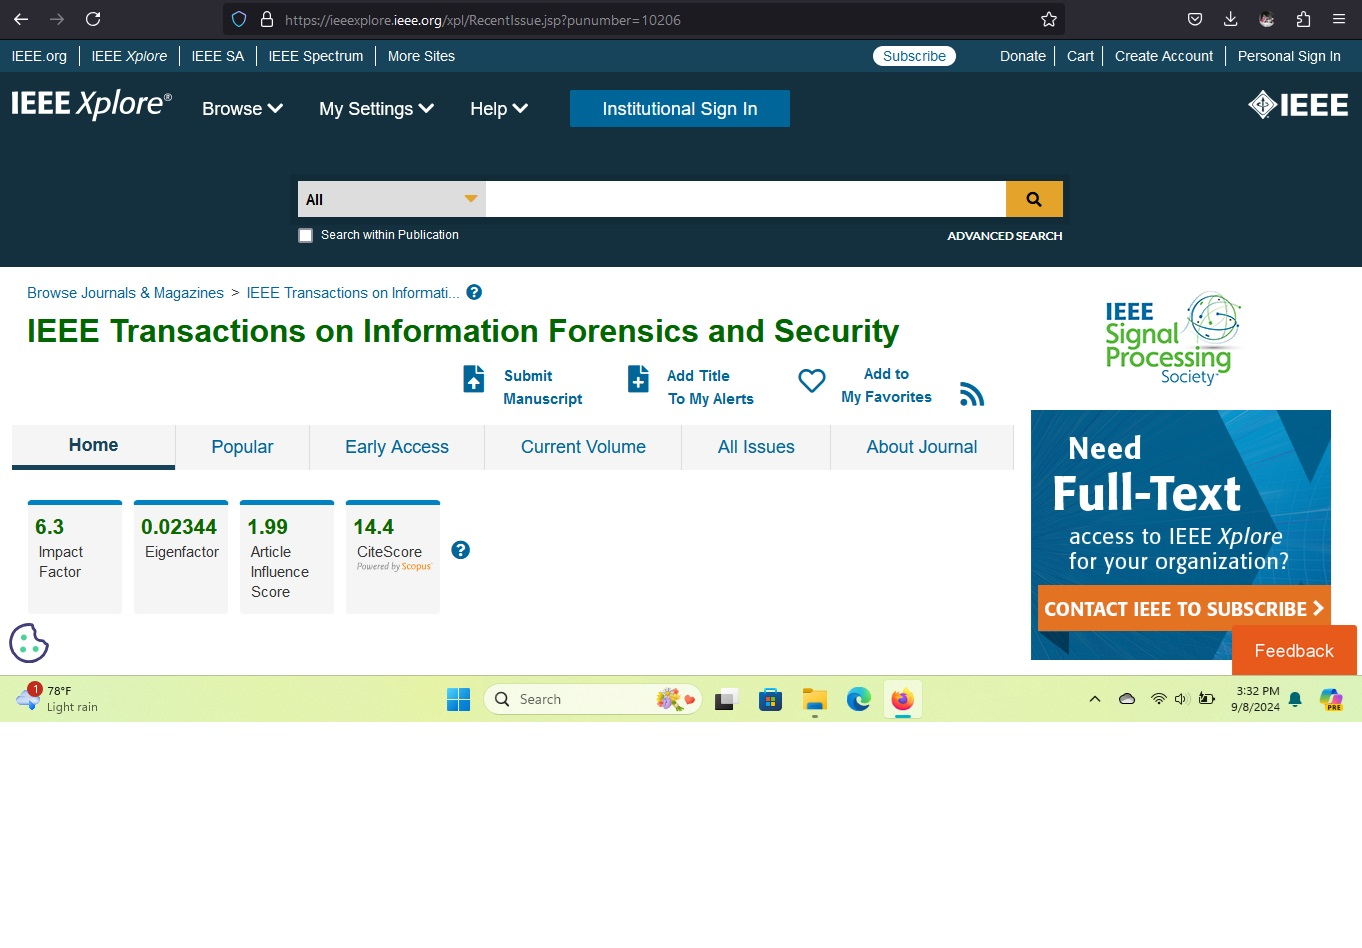
\includegraphics[width=0.8\textwidth]{content page2.jpg} % Replace with your actual image file
    \caption{Table of Contents from the selected venue}
    \label{fig:toc}
\end{figure}

\noindent The venue was chosen because it provides comprehensive coverage of the latest advancements in computer security and cybersecurity, aligning closely with my research interests. The table of contents image highlights relevant topics and ensures that the papers selected are highly pertinent to my study area.

\section{Process and Learning}
In this section, I will discuss the process and insights gained about conducting the research without delving into the content of the papers. 

\subsection{Process}
\begin{itemize}
    \item Identified relevant metrics and categories on Google Scholar.
    \item Narrowed down the search to \textbf{Engineering \& Computer Science} and specifically to \textbf{Computer Security \& Cryptography}.
    \item Evaluated papers based on relevance to the research area.
    \item Collected and reviewed papers to include in the journal.
\end{itemize}

\subsection{Learning}
\begin{itemize}
    \item Gained insights into effective search strategies for academic papers.
    \item Learned to utilize specific categories and subcategories to refine search results.
    \item Improved skills in organizing and documenting research findings.
\end{itemize}

\section{Raw Notes from Critical/Creative Reads}

\textbf{Raw Notes:}
\begin{itemize}
    \item Note 1: Summary of key findings from part1 ,part2 and part3
    \begin{figure}[ht]
        \centering
        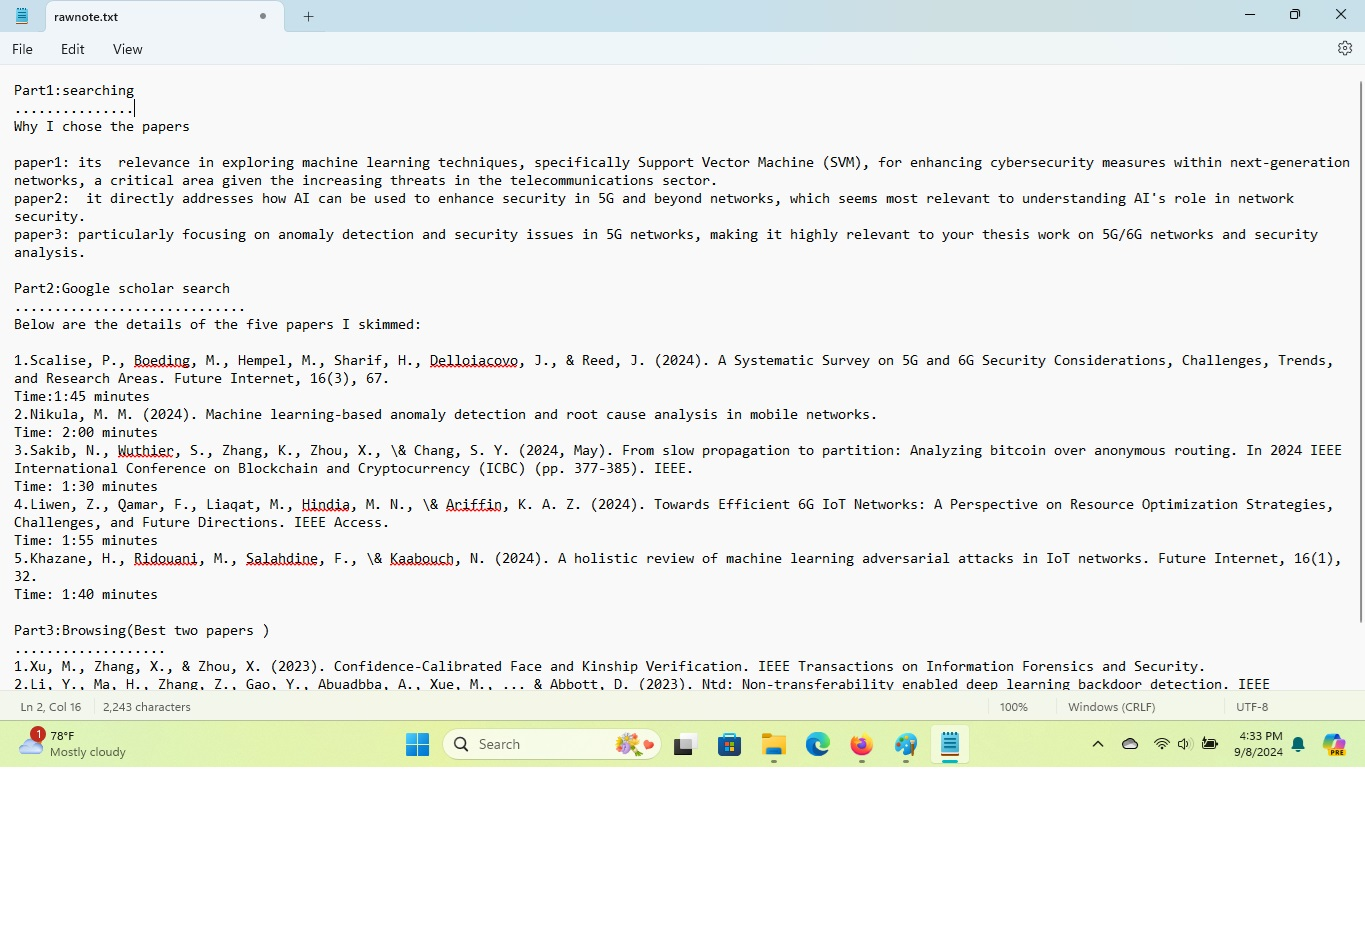
\includegraphics[width=0.8\textwidth]{rawnote1.jpg} % Replace with your actual image file
        \caption{Raw notes from critical/creative reads}
        \label{fig:notes}
    \end{figure}
    \item Note 2: key findings from Paper 1,Observations on methodology from Paper 2 and Insights on results from Paper 3 from part1
    \begin{figure}[ht]
        \centering
        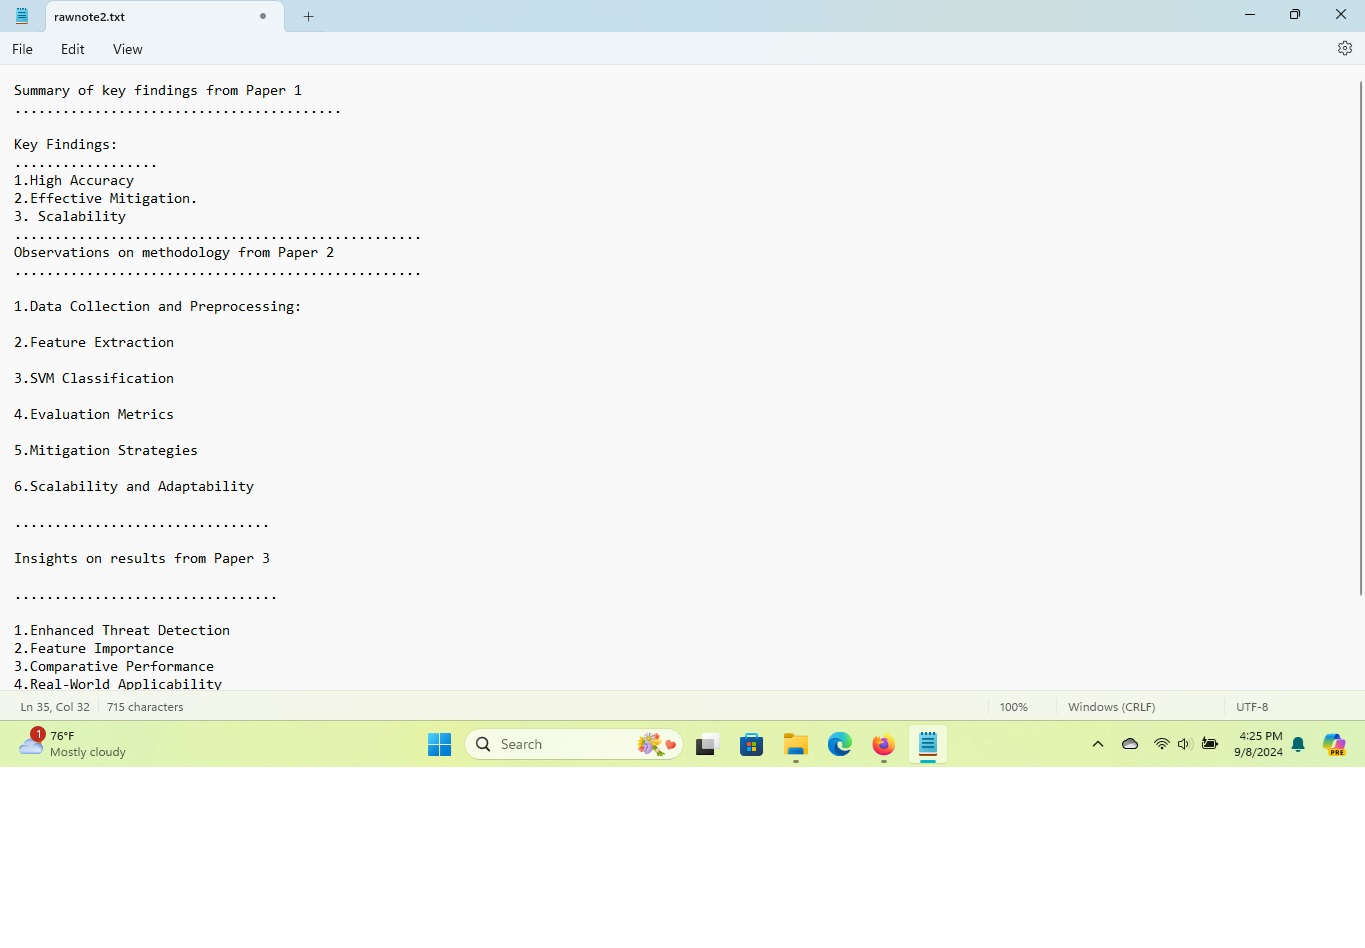
\includegraphics[width=0.8\textwidth]{note2.jpg} % Replace with your actual image file
        \caption{Raw notes for part1 from critical/creative reads}
        \label{fig:notes}
    \end{figure}
    
    \item Note 3: Timing and Decision notes from part3
    \begin{figure}[ht]
        \centering
        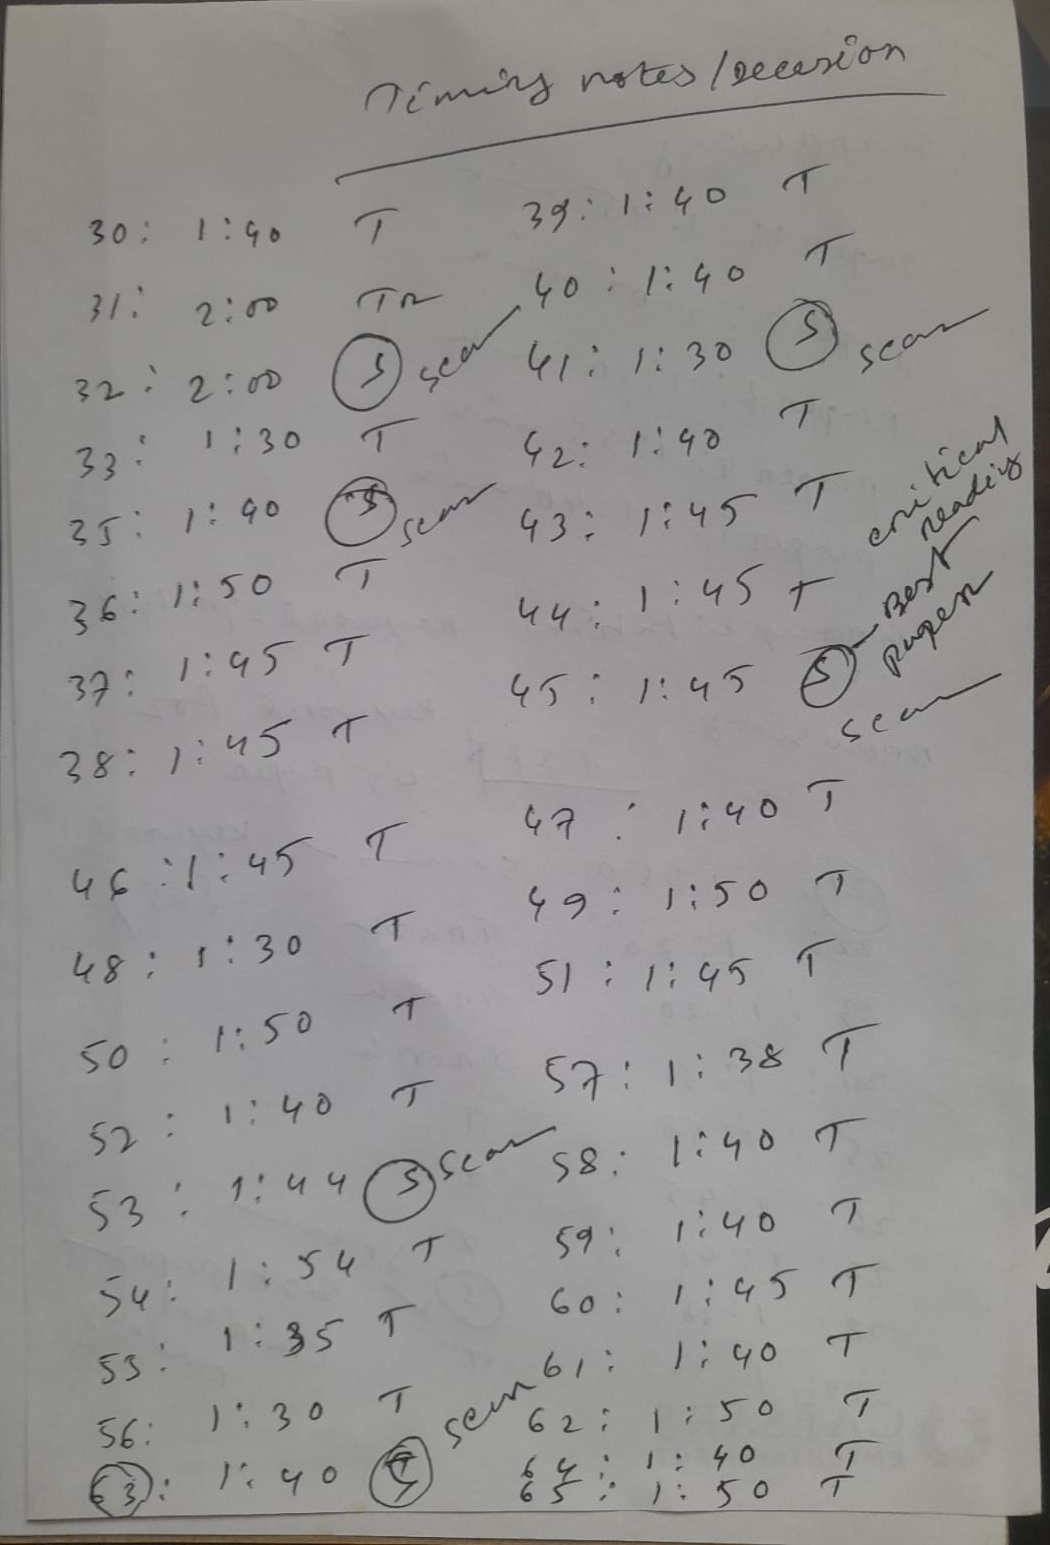
\includegraphics[width=0.8\textwidth]{handnote2.jpg} % Replace with your actual image file
        \caption{Handwritten notes on part3 from critical/creative reads}
        \label{fig:notes}
    \end{figure}
\end{itemize}

%\bibliographystyle{plain}  % Or another style
\nocite{*}  % This includes all entries from references.bib
\printbibliography
\end{document}
